
%(BEGIN_QUESTION)
% Copyright 2009, Tony R. Kuphaldt, released under the Creative Commons Attribution License (v 1.0)
% This means you may do almost anything with this work of mine, so long as you give me proper credit

Thermocouple-based temperature instruments work on the principle of measuring voltage output by a thermocouple:

$$\includegraphics[width=15.5cm]{i00386x01.eps}$$

If we try to simulate a thermocouple by using a precision potentiometer circuit to send a precise millivolt signal to a temperature instrument, however, the instrument will not register the way we might expect.  For instance, thermocouple tables for type J thermocouples tell us that 500 $^{o}$F corresponds to a voltage signal of 14.110 mV.  However, if we were to input this amount of signal voltage to a type J instrument, it would probably {\it not} register 500 $^{o}$F:

$$\includegraphics[width=15.5cm]{i00386x02.eps}$$

Describe what the problem is, and determine the amount of voltage we would have to ``dial up'' on the precision potentiometer in order to get the thermocouple instrument to register 500 $^{o}$F, assuming an ambient temperature of 72 $^{o}$F.

\vskip 20pt \vbox{\hrule \hbox{\strut \vrule{} {\bf Suggestions for Socratic discussion} \vrule} \hrule}

\begin{itemize}
\item{} Express in {\it general terms} how one could solve a problem such as this one.  In other words, think of a way to express a general step-by-step solution you could give to someone in the form of an instruction list, to show them how much voltage they would need to input to a temperature instrument to make it ``think'' it was connected to a thermocouple of any given temperature.
\item{} Should the thermistor in the compensation bridge possess a {\it positive} or a {\it negative} coefficient of resistance?
\end{itemize}

\underbar{file i00386}
%(END_QUESTION)





%(BEGIN_ANSWER)

In the calibration circuit, there is not a trace of thermocouple wire to be found.  Instead, all wires are made of copper.  This presents a problem for us because the temperature instrument has a reference junction compensation circuit built in, which at this point is compensating for a reference junction millivoltage that doesn't exist.  The instrument actually ``sees'' the series combination of the potentiometer's output voltage ($E_{potentiometer}$) and its own internally-generated compensation voltage ($E_{compensation}$), not the potentiometer voltage by itself.  This is why we cannot simply set the potentiometer to the millivoltage corresponding to our calibration temperature point and adjust the instrument to read the same.

\vskip 10pt

I'll let you figure out exactly how to work around this problem!

%(END_ANSWER)





%(BEGIN_NOTES)

To fix the problem, we must ``trick'' the compensation circuit so that it ``thinks'' it is actually compensating for something.  To do this, we must measure the temperature of the instrument's terminal block and calculate how much millivoltage a reference junction there would actually produce, then we offset our potentiometer setting by that amount at every calibration point.

\vskip 10pt

Since the desired voltage is 14.110 mV (corresponding to 500$^{o}$ F), subtracting the proper type-J millivoltage for a terminal block temperature of 72$^{o}$ F (1.134 mV) gives us:

$$14.110 \hbox{ mV} - 1.134 \hbox{ mV} = 12.976 \hbox{ mV}$$

%INDEX% Measurement, temperature: thermocouple millivoltage calibration

%(END_NOTES)


